
\section{Poisson Regression}
As a standard model for count data, a Poisson regression model is fit to establish a baseline to compare against neural networks.  The below output is the result from the general linear model function in base R, used on the training data, with the Poisson regression model specified by \texttt{family = "poisson"}.

\begin{verbatim}
## 
## Call:
## glm(formula = freqc ~ mag, family = "poisson", data = train)
## 
## Deviance Residuals: 
##      Min        1Q    Median        3Q       Max  
## -0.39403  -0.20754  -0.02925   0.08617   0.22166  
## 
## Coefficients:
##             Estimate Std. Error z value Pr(>|z|)    
## (Intercept)  13.0940     0.7242   18.08   <2e-16 ***
## mag          -2.0467     0.1474  -13.88   <2e-16 ***
## ---
## Signif. codes:  0 '***' 0.001 '**' 0.01 '*' 0.05 '.' 0.1 ' ' 1
## 
## (Dispersion parameter for poisson family taken to be 1)
## 
##     Null deviance: 373.0667  on 23  degrees of freedom
## Residual deviance:   0.7758  on 22  degrees of freedom
## AIC: Inf
## 
## Number of Fisher Scoring iterations: 3
\end{verbatim}

This shows that for every unit increase in magnitude, the expected difference in the logs of annual frequency is -2.0467.  The test error for this model, as will be for future models, was calculated by the mean squared error between predicted test values and actual test values. A plot of the data with the regression line is shown below:


\begin{figure}[H]
    \center
    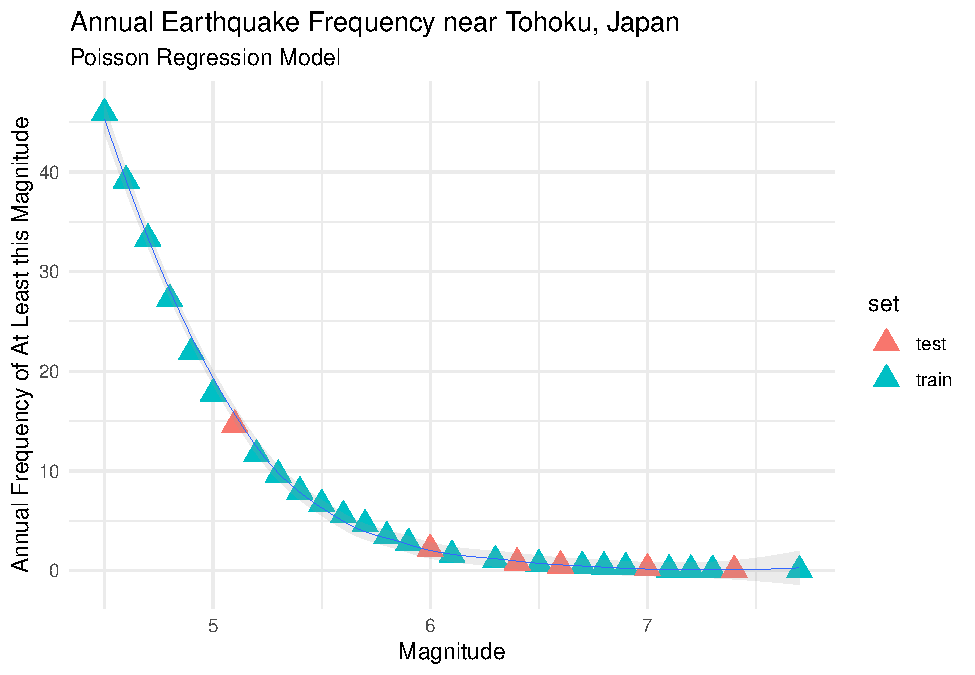
\includegraphics[width=0.75\linewidth]{Appendix_eq_files/figure-latex/unnamed-chunk-3-1.pdf}
   % \vspace{-10pt}
    \caption{\footnotesize{A Poisson regression line fit to the data.}}
    \label{tohoku_unfit}
\end{figure}

\begin{comment}

% latex table generated in R 4.2.2 by xtable 1.8-4 package
% Wed May  3 23:37:00 2023
\begin{table}[ht]
\centering
\begin{tabular}{rlr}
  \hline
 & Model & Test Error \\ 
  \hline
 & Poisson Regression &  0.1862851\\ 
   \hline
\end{tabular}
\end{table}

\end{comment}
